\documentclass[22pt]{report}
\usepackage[latin1]{inputenc}
\usepackage[francais]{babel}
\usepackage{amsmath,amssymb}
\usepackage{graphicx}



\begin{document}

Among applications which need to solve non-linear systems equations there is the Bairstow's Method, which enable to find two roots of a polynomial. \\
The problem is defined by this way, \\
we have $ P(x) = \sum_{k=0}^{n} a_k \cdot X^k$ \\
we put $ P(X) = (X^2 + B \cdot X + C) \cdot Q(X) + R(B,C) \cdot X + S(B,C)$
\\ and 

$f: \left[ \begin{array}{ccc}
    B \\
    C 
    \end{array} \right] \to 
\left[ \begin{array}{ccc}
  R(B,C) \\
  S(B,C) 
\end{array} \right]  $

\\
We have 
 $ f(B,C) = \left[ \begin{array}{ccc}
    0 \\
    0
    \end{array} \right] \Leftrightarrow P(X) = Q(X) \cdot (X^2 + B \cdot X + C)  $
\\ 
We start by choose B and C, and Suppose \\
$f(B + \delta B, C + \delta C) =  \left[ \begin{array}{ccc}
    0 \\
    0
    \end{array} \right]$
\\
In neighborhood of a root, a first-order Taylor series approximates the variation of R and S with respect the small changes  in B, C, we get a Newton-Raphson form  $ f(U) + H(U) \cdot V$ \\
which is\\ 

$ \begin{cases}
    R(B + \delta B, C + \delta C) = \frac{\delta R}{\delta B} \cdot \delta B + \frac{\delta R}{\delta C} \cdot \delta C   \\
S(B + \delta B, C + \delta C) = \frac{\delta S}{\delta B} \cdot \delta B + \frac{\delta S}{\delta C} \cdot \delta C   \\    
\end{cases}    
  $ \\

Finally, we get a Newton-Raphson Form ( $f(U) + J(U)\cdot V$ ) \\

with\\ 
$f(U) = \left[ \begin{array}{ccc}
    R(B, C) \\
    S(B, C) 
    \end{array} \right]$ \\

$V = \left[ \begin{array}{ccc}
    \delta B \\
    \delta C 
    \end{array} \right]$, and\\  

$ J(U) = \left[ \begin{array}{ccc}
    \frac{\delta R}{\delta B} \cdot \delta B & \frac{\delta R}{\delta C} \cdot \delta C \\
    \frac{\delta S}{\delta B} \cdot \delta B & \frac{\delta S}{\delta C} \cdot \delta C
    \end{array} \right] $
\\

To get the coefficients of J(U), we must put a second polynomial division \\
we put $ Q(X) = G(X) \cdot (X^2 + B \cdot X + C) + R_1 \cdot X + S_1$ \\
afterwards we get, 
$ \begin{cases}
  \frac{\delta R}{\delta B} = B \cdot R_1 - S_1\\
  \frac{\delta R}{\delta C} = -R_1\\
  \frac{\delta S}{\delta B} = C \cdot R_1\\
  \frac{\delta S}{\delta C} = -S_1\\ 
  \end{cases}$

After every iteration we get a new B and a new C by adding $\delta B$ and $\delta C$.

\\

Finally, we get Two roots of P thanks to B and C\\
Indeed, $ -B = X_+  + X_-$ and $C = X_+ \cdot X_-$\\
actually, we get $X_+$ and $X_-$ by solving $(X^2 + B \cdot X + C)$


Then, we have compared this method with a solving by newton Raphson in dimension 1

As well, we can optimize the algorithm by taking $B = \frac{a_{n-1}}{a_n}$ and $C = \frac{a_{n-2}}{a_n}$
\newpage
We have test those methods, and we have depended the average iteration of every algorithm.

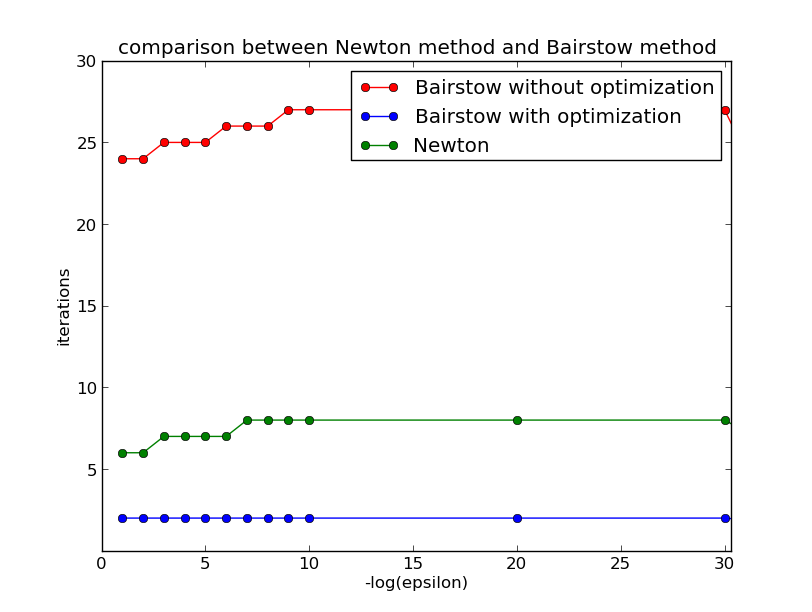
\includegraphics[scale = 0.5]{figure1.png} 

To Conclude, Bairstow's method optimized  is the most efficient and it is more automatic than the others. Moreover it find two roots unlike the newton raphson in 1 dimension which find a root. 

 
\end{document}
